% !TEX root = main.tex
% ======================================================================
% Chapter 5: Transformers as Conditional Compressors (ENHANCED)
% Enhanced with pedagogical improvements following Chapter 1 style
% ======================================================================

\chapter{Transformers as Conditional Compressors}
\label{ch:transformers}

\begin{keyinsight}
Transformers are not mysterious. They are \emph{conditional compressors}: models that factor a sequence into a product of predictable next-token distributions and learn to assign short codes to the likely continuations. The same mathematics that governs codelength (Chapter~\ref{ch:intro_information}) shapes attention, optimization, and sampling. When we talk about \emph{perplexity}, we are talking about \emph{bits per token}. When we talk about \emph{attention}, we are talking about \emph{data-dependent kernels} that retrieve and combine information to reduce codelength.
\end{keyinsight}

\vspace{0.6em}

\noindent This chapter builds transformers from the ground up, connecting each component to the compression view established in Chapter~\ref{ch:intro_information}. We will take our time with each concept, building intuition before introducing mathematics. By the end, you will understand not just \emph{how} transformers work, but \emph{why} each design choice matters for compression.

\begin{notationbox}
\textbf{Notation.} We write sequences as $x_{1:T} = (x_1,\dots,x_T)$ and contexts as $x_{<t} := x_{1:t-1}$. Bold lowercase denotes vectors ($\mathbf{q},\mathbf{k},\mathbf{v}\in\mathbb{R}^{d}$), bold uppercase matrices ($\mathbf{Q},\mathbf{K},\mathbf{V}\in\mathbb{R}^{T\times d}$), and plain symbols denote scalars. $\|\cdot\|$ is the Euclidean norm; $\softmax(\cdot)$ is rowwise softmax unless noted. We reserve $d_{\text{model}}$ for the residual stream width and $d_k$ for per-head key/query width.
\end{notationbox}

\vspace{1em}

% ======================================================================
% 5.1  Autoregression and codelength
% ======================================================================
\section{Autoregression and Codelength}
\label{sec:autoregression}

\subsection{Why predict one token at a time?}
\label{sec:why_autoregressive}

Before we dive into equations, let us think about the fundamental challenge. Suppose you want to compress a sentence like "The cat sat on the mat." You could try to encode the entire sentence at once, creating a single code for this particular seven-word sequence. But there are trillions of possible seven-word sentences, so your codebook would be enormous and mostly empty.

A better approach is to predict sequentially. You start with "The" and ask: what comes next? Maybe "cat" is likely, maybe "dog" is likely, but "xylophone" is very unlikely. You assign a probability to each possibility and use those probabilities to determine code lengths (remember from Chapter~\ref{ch:intro_information}: high probability means short code, low probability means long code).

Once you commit to "cat," you ask again: after "The cat," what comes next? Now "sat" becomes likely, "ran" is possible, but "cat" (repeating) is less likely. Your predictions improve because you have more context. This is the essence of autoregressive modeling: break the hard problem of predicting an entire sequence into a series of easier problems, each conditioned on what came before.

This approach has three key advantages. First, it is tractable: at each step you are just predicting one token from a vocabulary, not an entire sequence from an infinite space. Second, it reuses computation: the work you did to understand "The cat" helps you predict what comes after "The cat sat." Third, it matches how compression actually works: arithmetic coders encode symbols one at a time, with probabilities that can adapt based on what has been encoded so far.

\subsection{Breaking sequences into sequential predictions}
\label{sec:chainrule}

Now we can formalize this intuition. The chain rule of probability decomposes the joint likelihood of a sequence into a product of conditionals:
\begin{equation}
p(x_{1:T}) = \prod_{t=1}^{T} p(x_t \mid x_{<t}).
\label{eq:chainrule}
\end{equation}

This is not an approximation or a modeling choice. It is a mathematical identity that holds for any sequence. What makes it useful for modeling is that we can learn each conditional $p(x_t \mid x_{<t})$ separately, sharing parameters and patterns across positions.

Taking $-\log_2$ of both sides turns this into \emph{codelength}:
\begin{equation}
L(x_{1:T}) = -\sum_{t=1}^{T} \log_2 p(x_t \mid x_{<t}).
\label{eq:codelength}
\end{equation}

Let me show you why this matters with a concrete example. Consider the short sequence "The cat sat." Using a trained language model, we might get these probability assignments:

\begin{center}
\begin{tabular}{lccc}
\toprule
\textbf{Position} & \textbf{Token} & \textbf{Probability} & \textbf{Codelength (bits)} \\
\midrule
$t=1$ & "The" & $p(\text{The}) = 0.15$ & $-\log_2(0.15) = 2.74$ \\
$t=2$ & "cat" & $p(\text{cat} \mid \text{The}) = 0.08$ & $-\log_2(0.08) = 3.64$ \\
$t=3$ & "sat" & $p(\text{sat} \mid \text{The cat}) = 0.25$ & $-\log_2(0.25) = 2.00$ \\
\bottomrule
\end{tabular}
\end{center}

The total codelength for this sequence is $2.74 + 3.64 + 2.00 = 8.38$ bits. Notice how the codelength varies: "sat" gets a short code (2 bits) because after "The cat," the model correctly anticipates that a verb is likely. The word "cat" gets a longer code (3.64 bits) because after just "The," many nouns are possible and the model spreads probability across them.

This is compression in action. A model that understands language structure uses fewer bits on average than one that treats all words as equally likely. If we had used a uniform distribution over a vocabulary of fifty thousand words, each token would cost $\log_2(50000) \approx 15.6$ bits. Our model uses 8.38 bits for three tokens, or about 2.8 bits per token---a significant compression.

Minimizing expected codelength is exactly maximum likelihood estimation. When we train a transformer to minimize this sum, we are teaching it to compress sequences as efficiently as possible.

\subsection{Training versus generation: two modes, one model}

During \textbf{training}, we use a technique called \emph{teacher forcing}~\citep{williams_zipser_1989}. Each position $t$ sees the ground-truth context $x_{<t}$, which enables parallel computation of all $T$ conditionals. We compute the loss for every position simultaneously, take gradients, and update parameters. This is computationally efficient and provides clean learning signals.

During \textbf{inference} or generation, we cannot see the future. We must generate sequentially: sample $\hat{x}_1 \sim p(\cdot)$, feed it back as context, then sample $\hat{x}_2 \sim p(\cdot\mid \hat{x}_1)$, and so on. Each token depends on the tokens we have already generated, not on ground truth. Figure~\ref{fig:teacher_forcing} contrasts these regimes: parallel during training versus sequential at test time.

\begin{figure}[t]
\centering
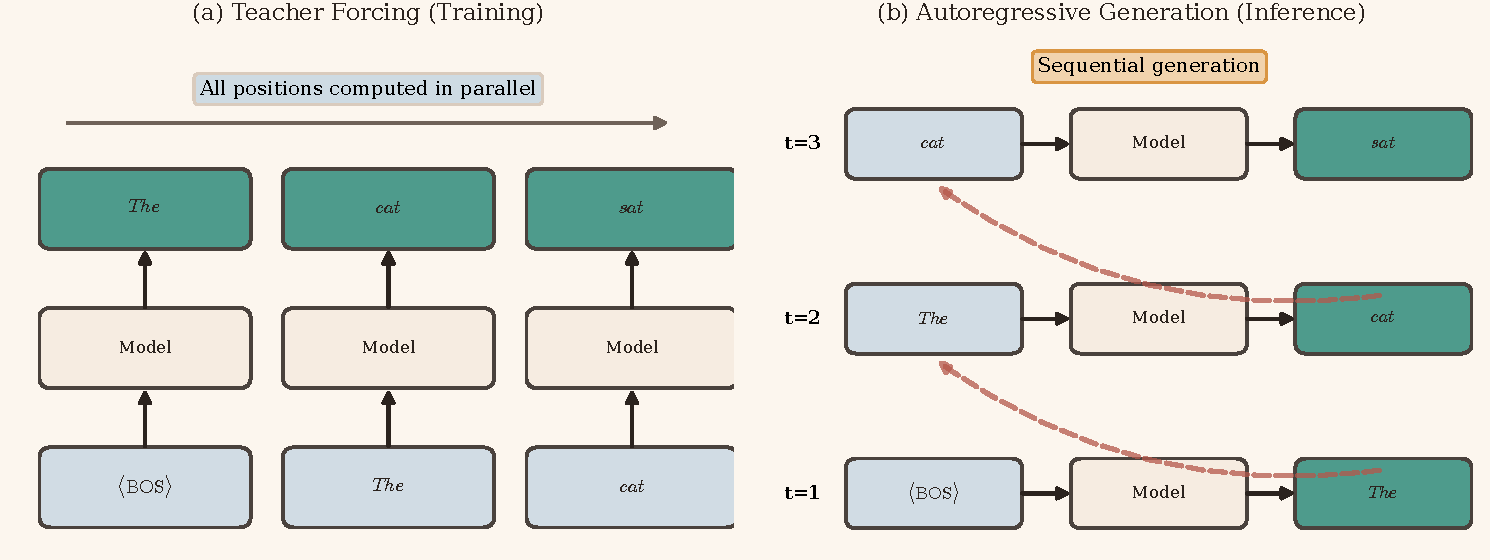
\includegraphics[width=0.92\textwidth]{code/figures/ch05_transformers_compressors/fig_5_2_teacher_forcing.pdf}
\caption{\textbf{Teacher forcing (left) vs.\ autoregressive generation (right).} In training, all conditionals are computed in parallel from ground-truth contexts; in generation, tokens are sampled and fed back sequentially (Section~\ref{sec:inference_sampling}).}
\label{fig:teacher_forcing}
\end{figure}

\vspace{0.6em}

\subsection{Perplexity, bits per token, and what they really mean}
\label{sec:perplexity_bits}

Perplexity is the exponential of average negative log-likelihood:
\begin{equation}
\mathrm{PPL} = \exp\!\Big(-\frac{1}{T}\sum_{t=1}^{T}\log p(x_t\mid x_{<t})\Big).
\end{equation}

In base-two units, the average \emph{bits per token} (bpt) equals $\frac{1}{T}\sum_t -\log_2 p(x_t\mid x_{<t})$. These are equivalent via $\mathrm{PPL}=2^{\text{bpt}}$.

You will often hear perplexity described as an "effective vocabulary size." This description is only strictly accurate for uniform distributions. The right mental model is more subtle: perplexity represents the \emph{geometric mean} of inverse probabilities. Let me show you what this means with actual numbers.

Suppose our model makes these four predictions:
\begin{center}
\begin{tabular}{lcc}
\toprule
\textbf{Token} & \textbf{Probability (correct)} & \textbf{Inverse probability} \\
\midrule
Token 1 & $0.80$ & $1/0.80 = 1.25$ \\
Token 2 & $0.10$ & $1/0.10 = 10.0$ \\
Token 3 & $0.50$ & $1/0.50 = 2.0$ \\
Token 4 & $0.90$ & $1/0.90 = 1.11$ \\
\bottomrule
\end{tabular}
\end{center}

The geometric mean of these inverse probabilities is $(1.25 \times 10.0 \times 2.0 \times 1.11)^{1/4} \approx 2.30$, giving perplexity of about 2.30.

What does this tell us? The model's average uncertainty is like choosing between two or three equally likely options, even though at individual positions it was very confident (tokens one and four) or quite uncertain (token two). The geometric mean captures typical uncertainty across positions, smoothing over the variations.

In bits per token, this same model achieves $\log_2(2.30) \approx 1.20$ bits per token. This is excellent performance. For reference, if your tokenizer's vocabulary has size $V=50{,}000$, a uniform guess would take $\log_2(50{,}000) \approx 15.6$ bits per token. Our model compresses to just 1.20 bits per token---more than a tenfold improvement over random guessing. This compression gain is the quantitative signature of learning.

Figure~\ref{fig:perplexity_bits} visualizes this relationship between perplexity and compression.

\begin{figure}[t]
\centering
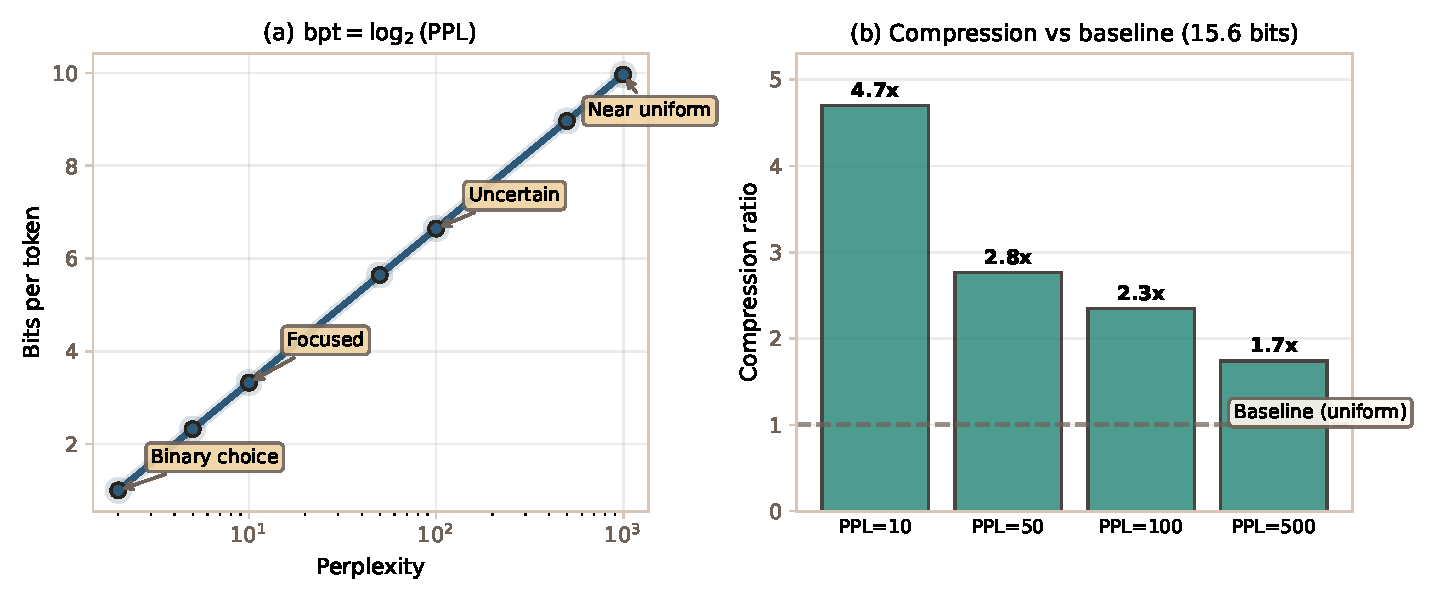
\includegraphics[width=0.95\textwidth]{code/figures/ch05_transformers_compressors/fig_5_7_perplexity_compression.pdf}
\caption{\textbf{Perplexity vs.\ bits per token.} Lower bpt means better compression (shorter expected codes). The right panel shows compression relative to a uniform $V$-way baseline.}
\label{fig:perplexity_bits}
\end{figure}

\vspace{0.6em}

\subsection{Exposure bias: what it is, where it bites, and why models cope}
\label{sec:exposure_bias}

There is an important mismatch between training and generation that we need to discuss honestly. During training, the model conditions on ground-truth histories. During generation, it conditions on its own sampled histories. When the model makes a mistake, that error becomes part of the context for future predictions, potentially triggering a cascade of compounding errors.

Here is a concrete example. Suppose the model generates "The chemical formula for water is NaCl" (confusing water with table salt). Now every subsequent token must make sense of this false premise. The model might continue with incorrect details, each error making the next error more likely. This is \textbf{exposure bias}: the model was never trained on its own mistakes, so it does not know how to recover from them.

For long sequences with strict constraints---like code that must compile, or formal proofs that must be valid---exposure bias can be a serious problem. A single syntax error at token one hundred might make token one hundred and one impossible to predict correctly, and the errors cascade.

However, two important truths coexist. First, this is a real failure mode that you should be aware of and design around when necessary. Techniques like scheduled sampling (gradually replacing some ground-truth context with model samples during training), sequence-level training objectives, or constrained decoding can help mitigate the problem.

Second, in practice, autoregressive language models trained with teacher forcing often generalize surprisingly well to generated contexts. Why? The learned distributions assign sufficient probability mass to neighborhoods around self-generated sequences that trajectories tend to remain in-distribution for modest horizons, especially when sampling conservatively (low temperature, nucleus sampling). The model has seen enough diverse text during training that its own reasonable outputs are not too far out of distribution.

The key is to acknowledge the risk and manage it: use appropriate sampling strategies (Section~\ref{sec:inference_sampling}), apply constrained decoding when validity is critical, and understand the limits of your model's robustness.

\vspace{0.6em}

\subsection{A word on universality---with the right caveats}
\label{sec:universality}

Autoregressive models are universal density approximators over sequences \emph{in the limit of sufficient capacity and data}: any computable distribution on finite strings can be approximated arbitrarily well by an autoregressive factorization with a large enough parametric class. This is not a claim that any particular transformer can model everything; it is a claim about asymptotics. Practical generalization depends on inductive biases (attention, residual pathways, normalization), optimization, and data quality. The universality theorem tells us there is no fundamental barrier, but engineering a system that actually works is where the art comes in.

\vspace{1.2em}

% ======================================================================
% 5.2  The attention mechanism
% ======================================================================
\section{The Attention Mechanism: Learning Where to Look}
\label{sec:attention}

\subsection{What problem does attention solve?}
\label{sec:attention_motivation}

Before we introduce any mathematics, let us understand the problem that attention solves. Imagine you are trying to predict the next word in this sentence: "The trophy didn't fit in the suitcase because it was too..."

To predict "big" or "small," you need to figure out what "it" refers to. Is "it" the trophy or the suitcase? The answer requires looking back at the context and understanding relationships between words that might be far apart.

How could we design a model to handle this? Consider three approaches:

\textbf{Option 1: Only look at the previous word.} This is too limited. Knowing that the previous word was "too" tells us almost nothing about whether "it" refers to the trophy or suitcase.

\textbf{Option 2: Average all previous word embeddings.} This is better because it incorporates the full context, but it is crude. It treats every previous word equally, so the word "because" (which is just a connector) gets the same weight as "trophy" (which is a potential referent for "it"). We are throwing away valuable information about which context words matter.

\textbf{Option 3: Dynamically weight previous words based on relevance.} This is what attention does. At the word "too" (when predicting the next word), we want the model to learn that "trophy" and "suitcase" are highly relevant (they are the potential referents), "because" is less relevant (it is just syntax), and most other words are even less relevant. We want to compute these relevance weights \emph{based on the content}---not with a fixed window or predetermined pattern, but by learning what to look for given what we are trying to predict.

Attention is a mechanism for content-based focusing. It learns to answer the question: given that I am trying to predict at position $t$, which previous positions should I pay attention to?

\subsection{Queries, keys, and values: the three ingredients}
\label{sec:qkv_intuition}

Attention uses three learned transformations of the input, which we call queries, keys, and values. These names come from information retrieval, and the analogy is helpful:

\textbf{Query:} "What am I looking for?" This is like typing a search query into a search engine. At position $t$, the query encodes what information would be useful for making a prediction at this position.

\textbf{Keys:} "What do I offer?" These are like document titles or metadata in a database. Each position $i$ has a key that advertises what information is available at that position. Keys are designed to match with queries.

\textbf{Values:} "What information do I actually contain?" These are like the actual document contents. Once we decide which positions are relevant (by matching queries to keys), we retrieve the values from those positions.

The separation into three components is crucial. We use queries and keys to determine \emph{where to look} (which positions are relevant), and then we use values to determine \emph{what to retrieve} (what information to extract from those positions). The learned projections allow the model to transform the same input embedding into different representations for different purposes.

Now we can write this mathematically. At position $t$, we compute:
\begin{align}
\mathbf{q}_t &= \mathbf{x}_t \mathbf{W}^Q \quad \text{(query: what I'm looking for)} \\
\mathbf{k}_i &= \mathbf{x}_i \mathbf{W}^K \quad \text{(key: what I offer, for all } i \le t \text{)} \\
\mathbf{v}_i &= \mathbf{x}_i \mathbf{W}^V \quad \text{(value: what I contain, for all } i \le t \text{)}
\end{align}

The matrices $\mathbf{W}^Q$, $\mathbf{W}^K$, and $\mathbf{W}^V$ are learned parameters. By learning different projections, the model can learn task-appropriate notions of "what to look for" and "where to find it."

\subsection{Computing attention: similarity, weights, and mixing}
\label{sec:attention_computation}

Once we have queries, keys, and values, we compute attention in three steps:

\textbf{Step 1: Compute similarity scores.} We measure how well the query at position $t$ matches the key at position $i$ using the dot product: $s_{ti} = \mathbf{q}_t^\top \mathbf{k}_i$. Higher dot product means higher similarity. We scale by $1/\sqrt{d_k}$ to prevent the scores from growing too large in high dimensions (we will explain why shortly):
\begin{equation}
s_{ti} = \frac{\mathbf{q}_t^\top \mathbf{k}_i}{\sqrt{d_k}}.
\end{equation}

\textbf{Step 2: Convert scores to weights using softmax.} We want a probability distribution over positions, so we apply softmax:
\begin{equation}
\alpha_{ti} = \frac{\exp(s_{ti})}{\sum_{j\le t}\exp(s_{tj})}.
\end{equation}

The weights $\alpha_{ti}$ tell us how much attention position $t$ pays to position $i$. They sum to one (over $i$), and positions with higher similarity get higher weight.

\textbf{Step 3: Mix the values according to the weights.} The output is a weighted average of the values:
\begin{equation}
\mathbf{o}_t = \sum_{i\le t}\alpha_{ti}\,\mathbf{v}_i.
\label{eq:attention_output}
\end{equation}

This is the core of attention. We have computed a context-dependent mixture of past values, where the mixture weights are determined by learned similarity between queries and keys.

\subsection{A detailed worked example}
\label{sec:attn_example}

Let us walk through a concrete example with actual numbers. Consider the partial sentence "The trophy didn't fit in the suitcase because it was too..."

At the position of the word "too," we want to predict the next word (often "big" or "small"). To make this prediction, the model needs to understand what "it" refers to.

Suppose we have $d_k = 64$ (the dimension of queries and keys). After computing queries and keys through the learned projections, we might get dot products like this:

\begin{center}
\begin{tabular}{lccc}
\toprule
\textbf{Position $i$} & \textbf{Token} & \textbf{Dot product} $\mathbf{q}_{\text{too}}^\top \mathbf{k}_i$ & \textbf{Scaled score} \\
\midrule
1 & "The" & $-1.6$ & $-1.6/\sqrt{64} = -0.20$ \\
2 & "trophy" & $7.2$ & $7.2/8 = 0.90$ \\
3 & "didn't" & $0.8$ & $0.8/8 = 0.10$ \\
4 & "fit" & $1.6$ & $1.6/8 = 0.20$ \\
5 & "in" & $-0.8$ & $-0.8/8 = -0.10$ \\
6 & "the" & $-1.6$ & $-1.6/8 = -0.20$ \\
7 & "suitcase" & $5.6$ & $5.6/8 = 0.70$ \\
8 & "because" & $-2.4$ & $-2.4/8 = -0.30$ \\
9 & "it" & $2.4$ & $2.4/8 = 0.30$ \\
10 & "was" & $0.0$ & $0.0/8 = 0.00$ \\
11 & "too" & $1.6$ & $1.6/8 = 0.20$ \\
\bottomrule
\end{tabular}
\end{center}

These raw dot products are consistent with what we would expect if the model has learned useful representations: "trophy" and "suitcase" (the potential referents) have high scores, while function words like "because" and "the" have low scores.

Now we apply softmax to get the attention weights (rounded to two decimals):
\begin{center}
\begin{tabular}{lcc}
\toprule
\textbf{Token} & \textbf{Scaled score} & \textbf{Attention weight} $\alpha$ \\
\midrule
"The" & $-0.20$ & $0.06$ \\
"trophy" & $0.90$ & $0.18$ \\
"didn't" & $0.10$ & $0.08$ \\
"fit" & $0.20$ & $0.09$ \\
"in" & $-0.10$ & $0.07$ \\
"the" & $-0.20$ & $0.06$ \\
"suitcase" & $0.70$ & $0.15$ \\
"because" & $-0.30$ & $0.05$ \\
"it" & $0.30$ & $0.10$ \\
"was" & $0.00$ & $0.07$ \\
"too" & $0.20$ & $0.09$ \\
\bottomrule
\end{tabular}
\end{center}

Notice that the model assigns the highest attention weights to "trophy" (18\%) and "suitcase" (15\%). This is exactly what we want: when predicting after "too," the model focuses on the two nouns that could be the referent of "it."

Finally, we compute the output by mixing the values according to these weights:
\begin{equation}
\mathbf{o}_{\text{too}} = 0.18 \cdot \mathbf{v}_{\text{trophy}} + 0.15 \cdot \mathbf{v}_{\text{suitcase}} + 0.10 \cdot \mathbf{v}_{\text{it}} + \ldots
\end{equation}

The output vector $\mathbf{o}_{\text{too}}$ is now a weighted combination that emphasizes the semantic features of "trophy" and "suitcase," which is exactly the information needed to predict whether the next word should be "big" (if "it" = trophy) or "small" (if "it" = suitcase).

This example shows the power of attention: by learning appropriate query, key, and value projections, the model can dynamically focus on relevant context without any explicit supervision about which words matter.

\subsection{Why scale by \texorpdfstring{$1/\sqrt{d_k}$}{1/sqrt(d\_k)}? A critical detail}
\label{sec:scaled_attention}

You might wonder why we divide the dot product by $\sqrt{d_k}$. This is not just a minor implementation detail---it is crucial for stable training in high dimensions.

When $\mathbf{q}$ and $\mathbf{k}$ are $d_k$-dimensional vectors with independent, standardized components, their dot product $\mathbf{q}^\top \mathbf{k}$ has variance proportional to $d_k$. As $d_k$ increases, the dot products spread out, and the softmax function becomes more extreme: most of the probability mass concentrates on a single position, and gradients vanish for all other positions.

Let me show you what happens with and without scaling. For a toy mental model, imagine a single query attending over a fixed number of positions, and suppose the unscaled dot products behave roughly like $\mathcal{N}(0,d_k)$. If you simulate such logits, you see something like:

\begin{center}
\begin{tabular}{lccc}
\toprule
$d_k$ & \textbf{Unscaled logits} & \textbf{Entropy} & \textbf{Max probability} \\
\midrule
1 & std $\approx$ 1 & 1.5 bits & 0.55 \\
10 & std $\approx$ 3.2 & 1.2 bits & 0.80 \\
100 & std $\approx$ 10 & 0.6 bits & 0.95 \\
500 & std $\approx$ 22 & 0.2 bits & $>$0.99 \\
\bottomrule
\end{tabular}
\end{center}

Without scaling, the distribution becomes nearly deterministic in high dimensions, attending to essentially a single position. This makes learning difficult because gradients are near zero for most positions.

With $1/\sqrt{d_k}$ scaling, we keep the logits at a consistent scale regardless of dimension (again, in this toy model):

\begin{center}
\begin{tabular}{lccc}
\toprule
$d_k$ & \textbf{Scaled logits} & \textbf{Entropy} & \textbf{Max probability} \\
\midrule
1 & std $\approx$ 1 & 1.5 bits & 0.45 \\
10 & std $\approx$ 1 & 1.5 bits & 0.45 \\
100 & std $\approx$ 1 & 1.5 bits & 0.45 \\
500 & std $\approx$ 1 & 1.5 bits & 0.45 \\
\bottomrule
\end{tabular}
\end{center}

These values are illustrative and aligned with the qualitative trends in Figure~\ref{fig:scaled_attention}.

The scaling stabilizes entropy across dimensions, which stabilizes gradients and makes optimization feasible. Figure~\ref{fig:scaled_attention} illustrates this effect visually.

\begin{figure}[t]
\centering
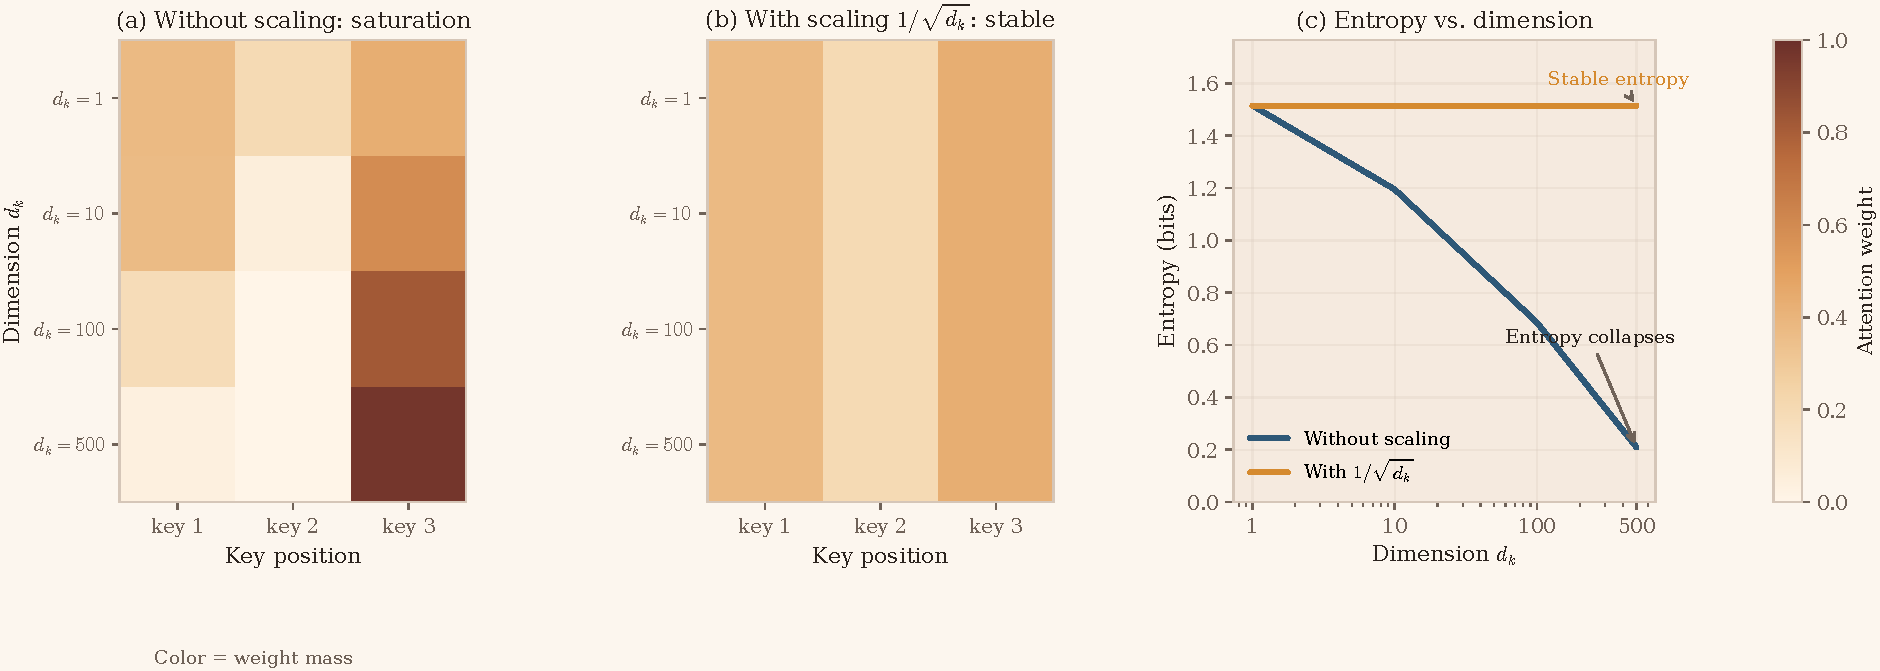
\includegraphics[width=0.92\textwidth]{code/figures/ch05_transformers_compressors/fig_5_4_scaled_attention.pdf}
\caption{\textbf{Why scale by $1/\sqrt{d_k}$?} Without scaling, logits grow with $\sqrt{d_k}$, saturating softmax; scaling stabilizes entropy across dimensions.}
\label{fig:scaled_attention}
\end{figure}

\subsection{Causal masking: enforcing the autoregressive structure}
\label{sec:causal_mask}

There is one more critical component: we must prevent the model from looking into the future. At position $t$, we can only attend to positions $i \le t$. Otherwise, the model could "cheat" during training by looking at future tokens.

We enforce this with a causal mask. Let $\mathbf{S}=\mathbf{Q}\mathbf{K}^\top/\sqrt{d_k}\in\mathbb{R}^{T\times T}$ be the matrix of all similarity scores. We define a mask $\mathbf{M}\in\{-\infty,0\}^{T\times T}$ where $\mathbf{M}_{ti}=0$ if $i\le t$ (allowed to attend) and $\mathbf{M}_{ti}=-\infty$ if $i > t$ (forbidden). Then:
\begin{equation}
\boldsymbol{\alpha}=\softmax(\mathbf{S}+\mathbf{M})\quad\text{(rowwise)},\qquad \mathbf{O}=\boldsymbol{\alpha}\,\mathbf{V}.
\label{eq:masked_softmax}
\end{equation}

Adding $-\infty$ before softmax ensures those positions get zero probability weight. The mask is not just a detail---it is the mechanism that implements the autoregressive factorization from Equation~\eqref{eq:chainrule}. Without it, we would not have a valid autoregressive model.

Figure~\ref{fig:qkv} shows the masked attention computation schematically.

\begin{figure}[t]
\centering
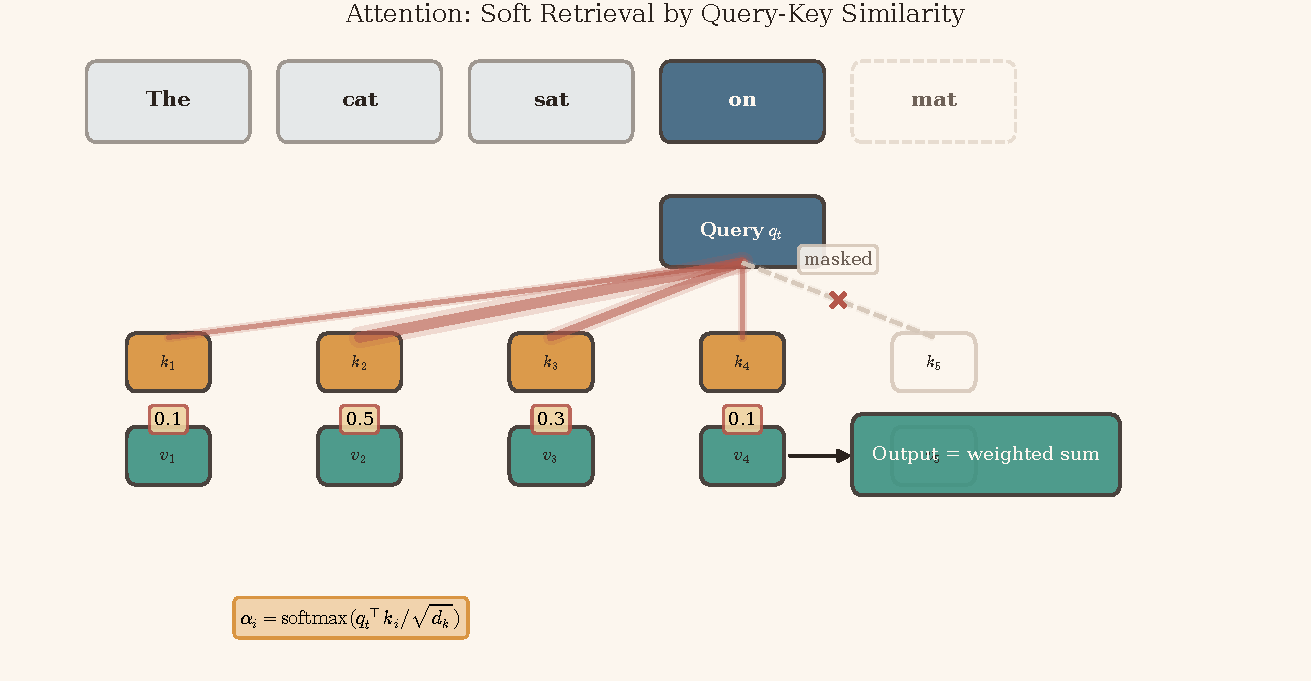
\includegraphics[width=0.92\textwidth]{code/figures/ch05_transformers_compressors/fig_5_3_attention_mechanism.pdf}
\caption{\textbf{Query--Key--Value attention with a causal mask.} A query at $t$ attends only to keys/values at $i\le t$. Connection thickness indicates attention weight.}
\label{fig:qkv}
\end{figure}

\begin{intuitionbox}
\textbf{Attention in one sentence.} Attention is content-based information retrieval: queries search over keys to find relevant past positions, then retrieve and mix the corresponding values.
\end{intuitionbox}

\vspace{1.2em}

% ======================================================================
% 5.3  Multi-head attention, FFNs, residuals, and normalization
% ======================================================================
\section{Multi-Head Attention, FFNs, Residuals, and Normalization}
\label{sec:architecture_core}

\subsection{The division of labor in a transformer layer}
\label{sec:division_of_labor}

Before we dive into the details of multi-head attention and feed-forward networks, let us understand the high-level architecture. A transformer layer has two main computational components, and they play complementary roles:

\textbf{Attention: Routing information.} Attention answers the question "where should I look?" It moves information between positions, gathering relevant context from different parts of the sequence. But attention only performs weighted averaging---it is linear in the values. It can route and combine information, but it cannot perform complex transformations.

\textbf{Feed-forward network: Transforming information.} The FFN answers the question "what should I compute?" It processes information at each position independently, applying nonlinear transformations. This is where the model does its "thinking"---pattern matching, memorization, and complex computations. But the FFN cannot move information between positions; it only transforms what is already at each position.

Together, they form an effective architecture: attention routes information to where it is needed, then the FFN transforms that information. This pattern repeats across many layers: route, transform, route, transform. The separation of concerns is not accidental---it is a key reason why transformers scale effectively.

\subsection{Multi-head attention: parallel specialists}
\label{sec:mha}

Single-head attention uses one set of projections to compute queries, keys, and values. Multi-head attention creates $H$ parallel "attention heads," each with its own learned projections:
\begin{equation}
\mathbf{Q}_h=\mathbf{X}\mathbf{W}_h^Q,\quad
\mathbf{K}_h=\mathbf{X}\mathbf{W}_h^K,\quad
\mathbf{V}_h=\mathbf{X}\mathbf{W}_h^V,\quad h=1,\dots,H.
\end{equation}

Each head computes attention independently:
\begin{equation}
\mathbf{O}_h=\softmax\Big(\frac{\mathbf{Q}_h\mathbf{K}_h^\top}{\sqrt{d_k}} + \mathbf{M}\Big)\,\mathbf{V}_h.
\end{equation}

Finally, we concatenate the outputs from all heads and project back to the residual stream dimension:
\begin{equation}
\mathrm{MHA}(\mathbf{X}) = [\mathbf{O}_1|\cdots|\mathbf{O}_H]\, \mathbf{W}^O.
\end{equation}

In practice, we typically choose $d_k = d_{\text{model}}/H$ so that concatenating $H$ heads returns a $d_{\text{model}}$-dimensional vector.

Why use multiple heads instead of one larger head? Empirically, different heads learn to specialize in different types of patterns. One head might focus on local syntax (attending to the previous few words). Another might track long-range dependencies like coreference (connecting pronouns to their antecedents). Another might attend to sentence boundaries or special delimiter tokens. By having multiple heads with their own parameters, we give the model the capacity to learn multiple different attention patterns simultaneously.

Think of it like having multiple specialized search engines: one for recent context, one for named entities, one for syntactic dependencies, and so on. Each head can learn its own notion of what "relevant context" means for its specialty.

\subsection{Feed-forward networks: the computational workhorse}
\label{sec:ffn}

After attention gathers context, each position passes through a feed-forward network. The FFN is applied identically and independently at every position:
\begin{equation}
\mathrm{FFN}(\mathbf{x}) = \mathbf{W}_2\,\phi(\mathbf{W}_1\,\mathbf{x} + \mathbf{b}_1)+\mathbf{b}_2,
\end{equation}
where $\phi$ is a nonlinearity (typically GELU or ReLU).

The FFN has a distinctive structure: it expands the dimension, applies nonlinearity, then contracts back. A typical pattern might be: $d_{\text{model}}=768 \rightarrow d_{\text{ff}}=3072 \rightarrow d_{\text{model}}=768$. This expansion creates a high-dimensional space where the network can represent complex computations, then projects the result back to the residual stream.

What does the FFN actually do? It performs pattern matching and memorization. During training, the FFN learns to recognize patterns in its input and produce appropriate outputs. For example, it might learn that when it sees features corresponding to "The capital of France," it should output features that promote "Paris" in the next-token prediction. The FFN is where much of the model's factual knowledge is stored---in the weights $\mathbf{W}_1$ and $\mathbf{W}_2$.

This is a useful rule of thumb, not a rigid law: factual information can also be represented in embeddings and expressed through attention pathways. But the FFN parameters account for a large fraction of a model's capacity, so they play a central role in memorization and transformation.

In terms of parameter count, FFNs typically account for about two-thirds of a transformer's parameters. The attention mechanism gets more conceptual focus, but the FFN provides most of the model's capacity. This is the "compute at the token site" that complements attention's "route across sites."

An intuitive analogy: if attention is like gathering ingredients from different places in your kitchen, the FFN is like actually cooking with those ingredients. Attention brings together relevant information; the FFN processes it to produce something useful.

\subsection{Residual pathways: the information highway}
\label{sec:residual_layernorm}

Transformers are built on residual connections, a technique borrowed from ResNets~\citep{he2016resnet}. Instead of replacing the input with the output of a layer, we \emph{add} the output to the input:
\begin{equation}
\mathbf{h}^{\ell+1}=\mathbf{h}^{\ell} + \mathrm{Sublayer}^{\ell}\!\big(\mathrm{Norm}(\mathbf{h}^{\ell})\big).
\label{eq:prenorm}
\end{equation}

This creates an "information highway" that runs through the network. Information can flow directly from the input to the output without being forced through every transformation. The attention and FFN layers make additive refinements to this signal, rather than having to reconstruct it from scratch at each layer.

Why is this important? Without residual connections, information must flow through a long chain of transformations: attention, FFN, attention, FFN, and so on. This is like a game of telephone---signals can degrade, gradients can vanish, and deep networks become very difficult to train. With residuals, we have a direct path that preserves information, while still allowing the model to make complex, multi-step refinements.

Layer normalization~\citep{ba2016layernorm} complements residuals by stabilizing the scale of activations. It normalizes features at each position:
\begin{equation}
\mathrm{LN}(\mathbf{h})=\gamma\odot \frac{\mathbf{h}-\mu}{\sigma} + \beta,\quad
\mu=\tfrac{1}{d}\sum_i h_i,\quad \sigma^2=\tfrac{1}{d}\sum_i(h_i-\mu)^2,
\end{equation}
with learned scale $\gamma$ and shift $\beta$. This prevents activations from exploding or vanishing as we stack layers.

The combination of residuals and normalization (typically in "pre-norm" configuration, as shown in Equation~\eqref{eq:prenorm}) is what makes it possible to train very deep transformers---models with dozens or even hundreds of layers.

\vspace{1.2em}

% ======================================================================
% 5.4  Positional encodings
% ======================================================================
\section{Positional Encodings}
\label{sec:positions}

Attention is permutation equivariant: if you scramble the input sequence, the attention weights just get scrambled the same way, but the computation is otherwise unchanged. This means the model has no inherent notion of position or order. For language, this is a problem: "dog bites man" and "man bites dog" would look identical.

We need to give the model information about position. There are several approaches, each with trade-offs.

\subsection{Absolute sinusoidal encodings}
\label{sec:sinusoid}

The classical approach from the original Transformer paper~\citep{vaswani2017attention} adds a deterministic position encoding $\mathbf{p}_t$ to each token embedding. The encoding uses sine and cosine functions with different frequencies:
\begin{align}
p_{t,2i} &= \sin(t / 10000^{2i/d_{\text{model}}}) \\
p_{t,2i+1} &= \cos(t / 10000^{2i/d_{\text{model}}})
\end{align}

The intuition is that different dimensions capture position at different scales. Low-frequency dimensions (slow-changing sines and cosines) capture coarse position---whether we are at the beginning, middle, or end of the sequence. High-frequency dimensions capture fine-grained position---the exact token index. This multi-scale representation allows the model to learn relative position relationships through linear combinations. Figure~\ref{fig:positional} illustrates this pattern.

\begin{figure}[t]
\centering
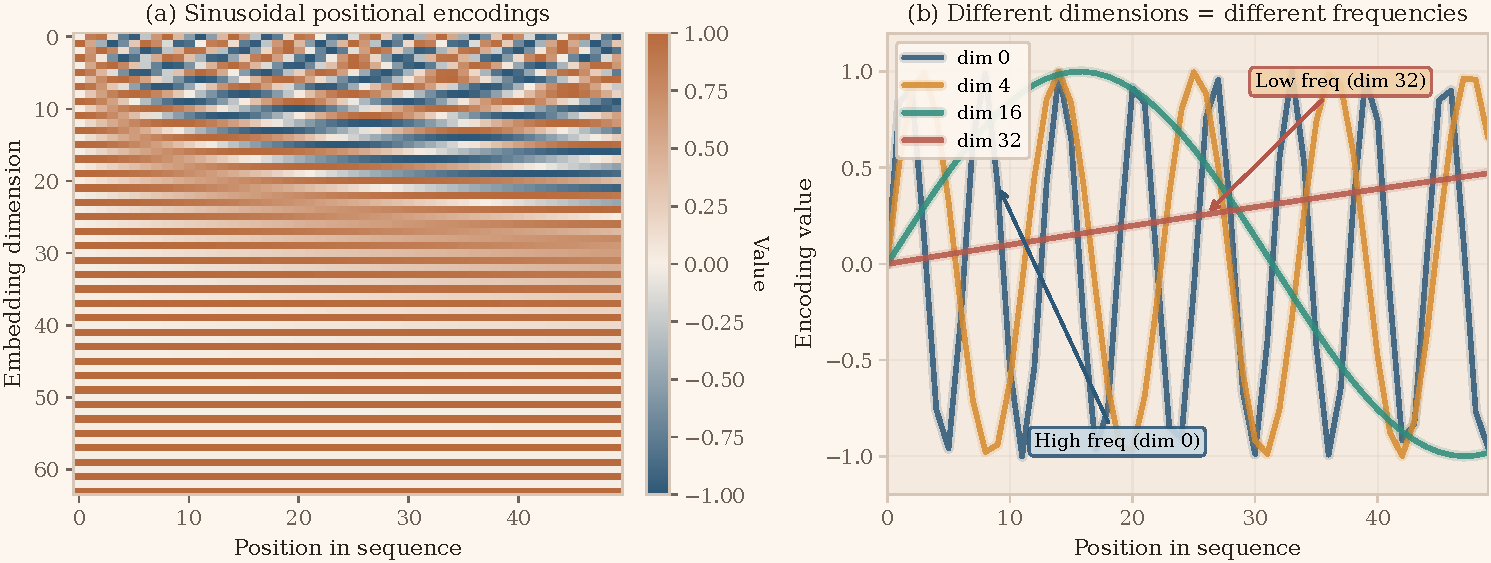
\includegraphics[width=0.92\textwidth]{code/figures/ch05_transformers_compressors/fig_5_6_positional_encodings.pdf}
\caption{\textbf{Sinusoidal positional encodings.} Low-frequency dimensions capture coarse location; high-frequency dimensions resolve fine detail.}
\label{fig:positional}
\end{figure}

Sinusoidal encodings work reasonably well and can extrapolate to lengths longer than those seen during training, though performance degrades on very long sequences if the model was not trained with length variation.

\subsection{Learned absolute embeddings}
\label{sec:learned_abs}

An alternative is to treat position as a categorical variable and learn an embedding for each position: $\mathbf{p}_t$ becomes a learned parameter looked up by index. This can fit the training range well, potentially better than fixed sinusoids, but extrapolation to longer sequences is often poor unless combined with other techniques.

\subsection{Relative and rotary encodings}
\label{sec:relative}

Modern large language models often use relative position encodings that modify the attention computation itself rather than just adding to embeddings. Two widely used approaches are:

\textbf{Rotary Position Embedding (RoPE)}~\citep{su2021rope} applies rotations to queries and keys such that their dot product depends on relative distance rather than absolute positions. This tends to extrapolate to longer contexts more gracefully than absolute encodings.

\textbf{ALiBi (Attention with Linear Biases)}~\citep{press2022alibi} adds a learned linear bias term that depends on distance into the attention scores. Despite being simpler than RoPE, it achieves good length extrapolation.

The key advantage of these methods is that they build the notion of relative position directly into the similarity computation, which is often more natural for language (we care that a pronoun is three words after its antecedent, not that one is at position 47 and the other at position 50).

\vspace{1.2em}

% ======================================================================
% 5.5  Training objectives
% ======================================================================
\section{Training Objectives}
\label{sec:training}

\subsection{Negative log-likelihood equals codelength}
\label{sec:nll_codelength}

We train transformers by maximizing the likelihood of the training data:
\begin{equation}
\max_\theta \sum_{(x_1,\ldots,x_T)} \sum_{t=1}^{T} \log p_\theta(x_t\mid x_{<t}).
\end{equation}

Equivalently, we minimize negative log-likelihood, which as we saw in Equation~\eqref{eq:codelength}, is exactly the codelength. This alignment is fundamental: the training objective directly optimizes compression. Every improvement in likelihood corresponds to better compression, which corresponds to learning more about the structure of the data.

During training, we use teacher forcing to compute all conditionals in parallel from ground-truth contexts. We typically add regularization: dropout, weight decay, and sometimes label smoothing. These can be understood as compression-aware priors in a PAC-Bayesian sense (we will explore this connection in Chapter~\ref{ch:pacbayes_mdl}).

\subsection{Tokenization: a brief note}
\label{sec:tokenization}

Before text can be processed by a transformer, it must be converted into tokens. Modern models use subword tokenization schemes like BPE (Byte Pair Encoding)~\citep{sennrich2016bpe} or WordPiece~\citep{schuster2012wordpiece}. These balance vocabulary size against sequence length: smaller vocabularies mean longer sequences but simpler distributions; larger vocabularies mean shorter sequences but more complex distributions. The choice affects bits per token directly. We defer a deeper discussion to Chapter~\ref{ch:highdim}.

\vspace{1.2em}

% ======================================================================
% 5.6  Inference and sampling
% ======================================================================
\section{Inference and Sampling: From Probabilities to Decisions}
\label{sec:inference_sampling}

Once we have trained a model, we need to actually generate text. This means converting the probability distribution $p_\theta(x_t\mid x_{<t})$ into a choice of next token. There are several strategies, each with different trade-offs between quality, diversity, and computational cost.

\subsection{A concrete scenario}
\label{sec:sampling_scenario}

Let us ground the discussion with a specific example. Suppose we are generating the continuation of "The capital of France is" and the model produces these probabilities:

\begin{center}
\begin{tabular}{lc}
\toprule
\textbf{Token} & \textbf{Probability} \\
\midrule
"Paris" & 0.850 \\
"paris" (lowercase) & 0.060 \\
"Lyon" & 0.028 \\
"the" & 0.010 \\
"Marseille" & 0.008 \\
"French" & 0.006 \\
... (49,994 other tokens) & $\sim$0.038 total \\
\bottomrule
\end{tabular}
\end{center}

This is a strongly peaked distribution: the model is quite confident that "Paris" is correct. But there is a long tail of alternative tokens with small probabilities. How we sample from this distribution makes a big difference in practice.

\subsection{Greedy decoding: always pick the most likely}
\label{sec:greedy}

The simplest strategy is greedy decoding: always pick $\arg\max_x p(x)$. In our example, we would deterministically select "Paris." Greedy decoding is fast, deterministic, and safe---it will never produce a very unlikely token.

The downside is that it can lead to repetitive or bland outputs. In more creative tasks (story generation, dialogue), greedy decoding tends to produce generic continuations. It also can get stuck in loops: once the model generates a phrase like "very very," it might keep repeating "very" because at each step, continuing the pattern has high probability.

Greedy decoding works well for factual tasks with clear correct answers---question answering, translation of simple sentences, code completion in obvious contexts. For open-ended generation, we usually want something more flexible.

\subsection{Temperature sampling: controlling randomness}
\label{sec:temperature_sampling}

Temperature sampling modifies the distribution before sampling. A temperature $\tau$ rescales probabilities (equivalently: divide logits by $\tau$):
\begin{equation}
p_\tau(x) \propto p(x)^{1/\tau}.
\end{equation}

With $\tau < 1$ (low temperature), we sharpen the distribution, making the model more confident and more likely to pick high-probability tokens. With $\tau > 1$ (high temperature), we flatten the distribution, increasing diversity at the cost of occasionally selecting unlikely tokens.

Let us see what happens to our example with different temperatures:

\begin{center}
\begin{tabular}{lccc}
\toprule
\textbf{Token} & $\tau=0.5$ (sharp) & $\tau=1.0$ (original) & $\tau=1.5$ (flat) \\
\midrule
"Paris" & 0.970 & 0.850 & 0.740 \\
"paris" & 0.018 & 0.060 & 0.087 \\
"Lyon" & 0.008 & 0.028 & 0.051 \\
"the" & 0.002 & 0.010 & 0.021 \\
Others & 0.002 & 0.052 & 0.101 \\
\bottomrule
\end{tabular}
\end{center}

At $\tau=0.5$, the model is even more confident in "Paris" (97\% probability). At $\tau=1.5$, the distribution is flatter: "Lyon" now has 5\% probability instead of 2.8\%, and low-probability tokens collectively have 10\% mass instead of 5\%.

For factual completion, we might use $\tau=0.7$ to reduce randomness. For creative writing, we might use $\tau=1.0$ or $\tau=1.2$ to increase variety. Very high temperatures ($\tau>2$) tend to produce incoherent text because the model starts sampling very unlikely tokens frequently.

\subsection{Top-k and nucleus sampling: adaptive truncation}
\label{sec:topk_nucleus}

Temperature adjusts the shape of the distribution but does not change the support---all tokens remain possible. Sometimes we want to explicitly truncate the distribution, keeping only the most probable tokens.

\textbf{Top-k sampling} keeps only the $k$ most probable tokens and renormalizes:
\begin{center}
\begin{tabular}{lcc}
\toprule
\textbf{Token} & \textbf{Original} & \textbf{Top-3 (renormalized)} \\
\midrule
"Paris" & 0.850 & $0.850 / 0.938 = 0.906$ \\
"paris" & 0.060 & $0.060 / 0.938 = 0.064$ \\
"Lyon" & 0.028 & $0.028 / 0.938 = 0.030$ \\
Others & 0.062 & 0 (excluded) \\
\bottomrule
\end{tabular}
\end{center}

Top-k works well when you want to cap the maximum risk---you will never sample a token outside the top $k$. Typical values are $k=20$ to $k=50$. The downside is that $k$ is fixed: for peaked distributions (like our "Paris" example), keeping 50 tokens might include many irrelevant options; for flat distributions, keeping only 20 might exclude reasonable alternatives.

\textbf{Nucleus sampling (top-p)}~\citep{holtzman2019curious} adapts to the distribution shape. Instead of keeping a fixed number of tokens, it keeps the smallest set $S$ such that $\sum_{x \in S} p(x) \ge p_0$, where $p_0$ is a threshold (typically 0.9 to 0.95).

For our example with $p_0=0.90$:
\begin{center}
\begin{tabular}{lcc}
\toprule
\textbf{Token} & \textbf{Probability} & \textbf{Cumulative} \\
\midrule
"Paris" & 0.850 & 0.850 \\
"paris" & 0.060 & 0.910 (exceeds threshold) \\
\midrule
Included & \multicolumn{2}{c}{"Paris", "paris"} \\
\bottomrule
\end{tabular}
\end{center}

Only two tokens are needed to reach 90\% cumulative probability, so nucleus sampling would only sample from {"Paris", "paris"}. In a flatter distribution, more tokens would be included. This adaptive behavior makes nucleus sampling work across different contexts.

\subsection{Beam search: exploring multiple paths}
\label{sec:beam}

All the sampling methods above are local: at each step, we pick one token and commit to it. Beam search maintains multiple candidate sequences (the "beam") and explores them in parallel.

At each step, for each sequence in the beam, we consider all possible next tokens, score each extension by cumulative log-probability, and keep the top $B$ sequences (where $B$ is the beam width). This continues until all sequences reach an end token or maximum length.

Beam search is useful for tasks where there is a clear quality metric to optimize (like BLEU score in translation). It tends to find high-probability sequences. However, beam search can also lead to generic outputs in creative tasks because it favors safe, high-likelihood continuations. For dialogue or story generation, beam search often produces boring text.

Typical beam widths are $B=4$ to $B=8$. Larger beams improve coverage but increase computational cost linearly.

\subsection{Choosing a sampling strategy: a decision guide}
\label{sec:sampling_choice}

Here is a compact guide for choosing a sampling strategy:

\begin{center}
\small
\begin{tabular}{p{0.18\textwidth} p{0.28\textwidth} p{0.18\textwidth} p{0.22\textwidth}}
\toprule
\textbf{Strategy} & \textbf{When to use} & \textbf{Typical setting} & \textbf{Main risk} \\
\midrule
Greedy & Factual tasks, slots, extraction & (deterministic) & Repetition, blandness \\
Temperature & Fine-tuning diversity & $\tau=0.7$--$1.1$ & Too confident or incoherent \\
Top-k & Fixed diversity cap & $k=20$--$50$ & Misses rare valid tokens \\
Nucleus & Adaptive diversity & $p=0.9$--$0.95$ & Can exclude valid tails \\
Beam & Metric-driven tasks & width $4$--$8$ & Generic outputs \\
\bottomrule
\end{tabular}
\end{center}

In practice, many applications combine strategies: nucleus sampling with $p=0.95$ and temperature $\tau=0.9$ gives adaptive truncation with slightly sharpened probabilities, balancing quality and diversity.

Figure~\ref{fig:sampling_schemes} visualizes these different sampling methods applied to the same model distribution.

\begin{figure}[t]
\centering
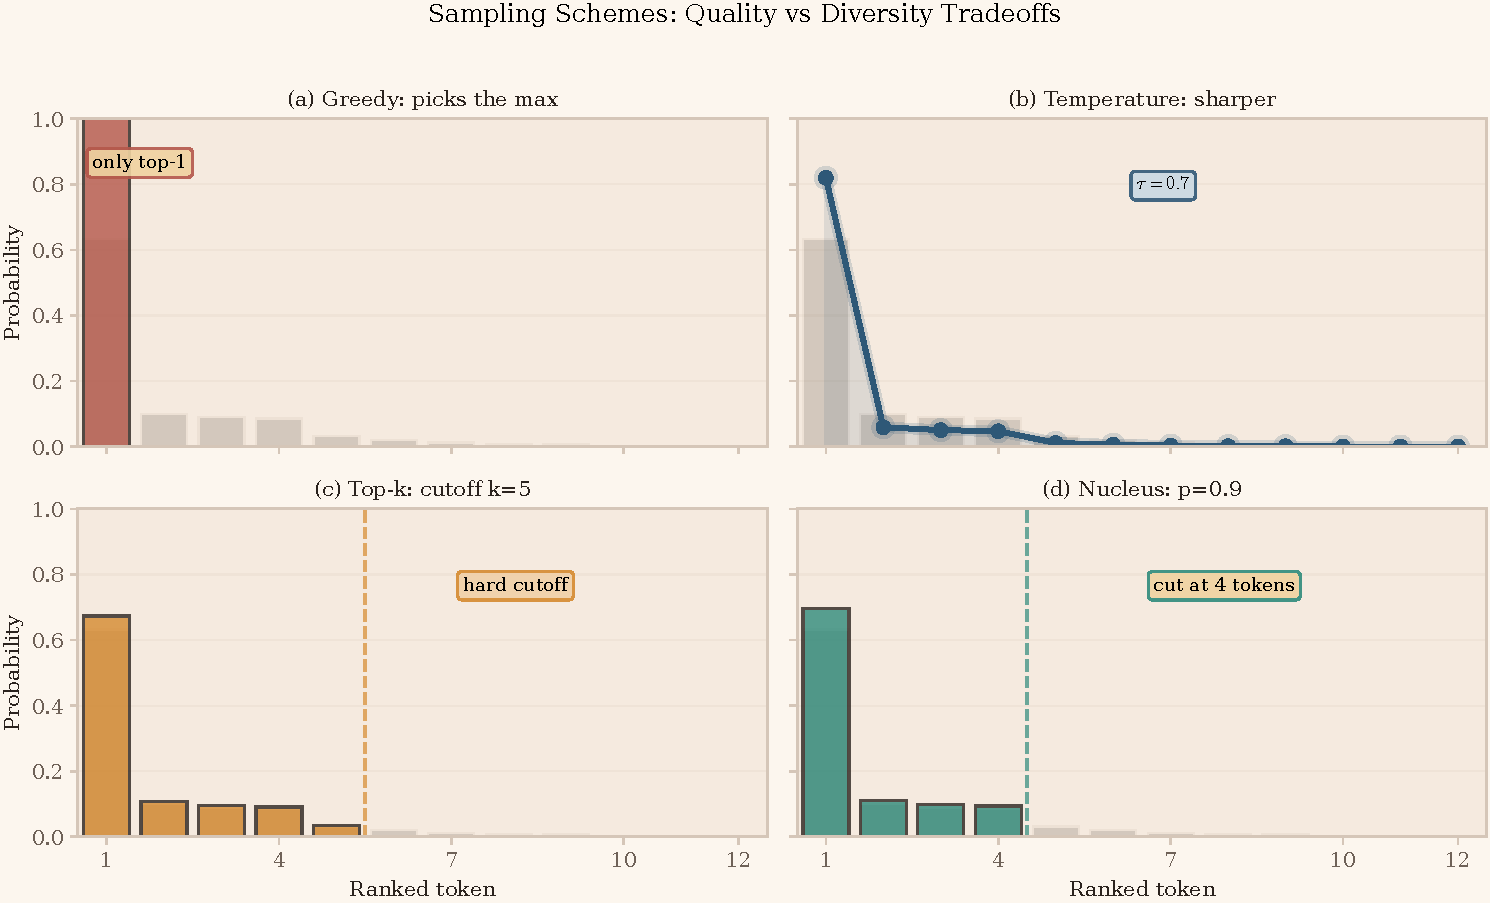
\includegraphics[width=0.95\textwidth]{code/figures/ch05_transformers_compressors/fig_5_8_sampling_schemes.pdf}
\caption{\textbf{Sampling schemes.} Greedy, temperature, top-$k$, and nucleus sampling compared on the same model distribution.}
\label{fig:sampling_schemes}
\end{figure}

\subsection{Constrained decoding for validity}
\label{sec:validity_constraints}

When outputs must satisfy formal constraints---like valid JSON, grammatical code, or structured data---we can use constrained decoding. This masks out invalid tokens at each step, ensuring the output conforms to a grammar or schema. Libraries like Guidance or LMQL implement this efficiently. When constraints are complex, post-hoc validation and repair are pragmatic alternatives. We defer production details to Chapter~\ref{ch:systems}.

\vspace{1.2em}

% ======================================================================
% 5.7  What transformers compress
% ======================================================================
\section{What Transformers Compress: An Empirical Bits/Token Lens}
\label{sec:what_compress}

\subsection{A minimal worked compression example}
\label{sec:compression_example}

Let us make the compression view concrete with actual measurements. We evaluate a trained decoder-only language model on three different types of text:

\textbf{Curated encyclopedia text:} Well-edited, formal English. The model achieves approximately 2.0 to 3.5 bits per token. The text has clear structure, standard vocabulary, and predictable patterns (formal tone, topic coherence). The model compresses effectively because its training data includes similar text.

\textbf{Programming code:} Python or JavaScript source code. The model achieves approximately 1.8 to 3.0 bits per token, often better than natural language. Why? Code has very strong local structure: if you see "for i in range(", the next token is almost certainly a number or variable name, followed by ")". Indentation, keywords, and syntax create highly predictable patterns. The model leverages this regularity for better compression.

\textbf{Random text:} We take the same vocabulary and generate uniformly random token sequences. The irreducible baseline here is $\log_2(V)$ bits per token (for $V=50{,}000$, this is about 15.6 bits per token): there is no structure to exploit, so no model can beat that on uniform randomness. In practice, a trained language model typically lands near this baseline and often slightly above it, because its learned distribution is not uniform and cannot match pure noise.

These numbers vary by tokenizer, data, and model size, but the pattern is stable: where structure exists and the model's inductive biases fit, compression is strong; where structure is absent, bits per token rises to the uniform baseline.

This is exactly what we expect from Chapter~\ref{ch:intro_information}: compression is learning. Better models find shorter codes by discovering patterns. The bits per token metric quantifies how much structure the model has successfully captured.

\subsection{Why this architecture works: an information-theoretic perspective}
\label{sec:why_transformer_works}

From the compression viewpoint, every component serves a purpose:

Attention is a content-addressable retrieval mechanism that gathers relevant context dynamically. It reduces codelength by finding the right information to condition on, rather than averaging over everything equally.

Feed-forward networks are nonlinear computers that transform retrieved information into useful predictions. They store learned patterns and perform the actual "thinking."

Residual streams preserve information across depth, ensuring that useful signals from early layers can inform later predictions without degradation.

Layer normalization stabilizes the learning dynamics, allowing us to stack many layers without optimization failure.

Together, they form an efficient conditional compressor: route (attention), compute (FFN), preserve (residuals), stabilize (norm). The empirical fact that bits per token drops as models scale (Chapter~\ref{ch:scaling}) is the quantitative signature of this architecture succeeding at better compression.

\vspace{1.2em}

% ======================================================================
% 5.8  Architectural variants
% ======================================================================
\section{Architectural Variants: When to Use Which}
\label{sec:variants}

\subsection{Decoder-only (GPT-style)}
Use when the task is next-token prediction or free-form generation conditioned on a prompt. This architecture has a simple causal stack, natural autoregressive structure, and efficient KV caching for long generations. Examples: dialogue, code completion, story generation.

\subsection{Encoder-only (BERT-style)}
Use when you need representations of entire inputs for classification, retrieval, or span labeling. Bidirectional context at every token gives rich representations. Examples: sentence embedding, named entity recognition, document reranking.

\subsection{Encoder--decoder (sequence-to-sequence)}
Use when input and output are distinct modalities or when you want a bottlenecked conditioning pathway. The encoder builds a task-specific representation; the decoder conditions on it to generate. Examples: translation, summarization, instruction-to-code.

\vspace{1.2em}

% ======================================================================
% 5.9  Compute and memory costs
% ======================================================================
\section{Compute and Memory Costs}
\label{sec:complexity}

Self-attention scales as $\mathcal{O}(T^2 d_{\text{model}})$ per layer due to the all-pairs similarity computation. Feed-forward networks scale as $\mathcal{O}(T d_{\text{model}} d_{\text{ff}})$. For long sequences, attention is the bottleneck; for short sequences, FFNs dominate.

During training, we must store activations for backpropagation. During inference in decoder-only models, we cache keys and values to avoid recomputing attention for previously generated tokens. This trades memory ($\mathcal{O}(T d_{\text{model}})$) for speed---a worthwhile trade in most interactive applications.

Efficient attention variants (sparse patterns, low-rank approximations, chunking) reduce the quadratic cost at the expense of approximation quality. Use them when $T$ is very large and you can tolerate some degradation.

\vspace{1.2em}

% ======================================================================
% 5.10  Why transformers beat RNNs
% ======================================================================
\section{Why Transformers Beat RNNs}
\label{sec:why_beats_rnns}

Transformers have largely replaced RNNs for sequence modeling. Two decisive advantages explain why:

\textbf{Parallelism.} RNNs process sequences sequentially, one step at a time. Transformers compute all positions in parallel during training (via teacher forcing), enabling large-batch optimization on modern hardware. This unlocks the scale that drives performance.

\textbf{Long-range credit assignment.} RNNs backpropagate through time, accumulating products of Jacobians that often vanish or explode. Transformers provide direct paths between any two positions via attention, making it easier to learn long-range dependencies. Gradients flow cleanly even between distant tokens.

These advantages compound: parallelism enables scaling to huge models and datasets; long-range credit enables learning complex patterns. Together, they have made transformers the dominant architecture for language and increasingly for other modalities.

\vspace{1.2em}

% ======================================================================
% 5.11  Pause and consolidate
% ======================================================================
\section*{Pause and Consolidate}
\label{sec:pause}

We have covered a lot of ground. If you are feeling somewhat overwhelmed, that is completely normal---transformers pack many interacting components into a single architecture. The key is to hold onto the central thread: \emph{transformers are conditional compressors that predict to compress}.

Here are the essential ideas to take away. Autoregressive modeling breaks sequence prediction into manageable steps, each predicting one token given the past. Attention dynamically focuses on relevant context using learned queries and keys, then retrieves values. Multi-head attention and FFNs divide labor: attention routes information, FFNs transform it. Residuals and normalization enable deep composition. The training objective minimizes codelength, which is exactly maximum likelihood.

When we generate, we convert probabilities into tokens using sampling strategies that trade off quality and diversity. The bits per token metric quantifies compression quality, which directly reflects how much the model has learned about the structure of the data.

If any specific component still feels unclear, go back and reread that section. These concepts build on each other, and understanding each piece solidly will make the rest easier. The time you invest now will pay off throughout the rest of the book.

The most important equation to remember is Equation~\eqref{eq:codelength}: codelength equals the sum of negative log probabilities. Everything else serves this goal.

\vspace{2em}

% ======================================================================
% 5.12  Exercises
% ======================================================================
\section*{Exercises}

\textbf{1. Chain rule to codelength ($\star$).} Starting from Eq.~\eqref{eq:chainrule}, derive Eq.~\eqref{eq:codelength}. Explain why minimizing average codelength is the same as minimizing cross-entropy.

\vspace{0.3cm}

\textbf{2. Scaled attention saturation ($\star$).} Simulate three dot-product scores with $d_k\in\{16,64,256\}$. Show that without $1/\sqrt{d_k}$ the softmax distribution saturates as $d_k$ grows; with scaling, entropies remain comparable.

\vspace{0.3cm}

\textbf{3. Attention as retrieval ($\star$).} Take the sentence "The trophy didn't fit because it was too..." Manually design plausible query and key vectors such that attention at "too" assigns high weight to "trophy." Explain your design choices.

\vspace{0.3cm}

\textbf{4. Causal masking ($\star$).} Implement masked softmax as in Eq.~\eqref{eq:masked_softmax}. Visualize the attention matrix with and without a causal mask.

\vspace{0.3cm}

\textbf{5. Bits/token vs.\ sampling strategy ($\star\star$).} For a trained language model, sweep $p_0\in[0.8,0.98]$ in nucleus sampling. Measure bits per token of the resulting samples under the model and report diversity (unique $n$-grams). Discuss the Pareto frontier.

\vspace{0.3cm}

\textbf{6. Perplexity reality check ($\star$).} Given a vocabulary $V=50{,}000$, compute the uniform baseline bits per token and compare to your model's bits per token on held-out text. Interpret the ratio as compression gain.

\vspace{0.3cm}

\textbf{7. Temperature effects ($\star\star$).} Take a model distribution with one high-probability token (0.8) and many low-probability tokens. Apply temperatures $\tau \in \{0.5, 1.0, 2.0\}$ and visualize the resulting distributions. Generate samples and characterize the qualitative differences.

\vspace{0.3cm}

\textbf{8. Position encoding ablation ($\star\star$).} Train a small transformer with and without positional encodings. Evaluate on a task where order matters (e.g., arithmetic). Quantify the performance gap.

\vspace{0.3cm}

\textbf{9. Residual stream ablation ($\star\star$).} Remove residual connections and attempt to train. Diagnose failure modes (optimization vs.\ expressivity) and connect to theory.

\vspace{0.3cm}

\textbf{10. Exposure bias stress test ($\star\star\star$).} Create a synthetic grammar with strict long-range constraints. Compare greedy vs.\ nucleus vs.\ constrained decoding. Quantify failure cascades.

\vspace{2em}

% ======================================================================
% References
% ======================================================================
\section*{References}

{\small
\begin{hangparas}{.25in}{1}
\noindent
Ba, J. L., Kiros, J. R., \& Hinton, G. E. (2016). Layer Normalization. \emph{arXiv:1607.06450}.

\noindent
Bahdanau, D., Cho, K., \& Bengio, Y. (2014). Neural Machine Translation by Jointly Learning to Align and Translate. \emph{arXiv:1409.0473}.

\noindent
Fan, A., Lewis, M., \& Dauphin, Y. (2018). Hierarchical Neural Story Generation. \emph{ACL}.

\noindent
Gehring, J., Auli, M., Grangier, D., \& Dauphin, Y. (2017). Convolutional Sequence to Sequence Learning. \emph{ICML}.

\noindent
He, K., Zhang, X., Ren, S., \& Sun, J. (2016). Deep Residual Learning for Image Recognition. \emph{CVPR}.

\noindent
Holtzman, A., Buys, J., Du, L., Forbes, M., \& Choi, Y. (2019). The Curious Case of Neural Text Degeneration. \emph{ICLR}.

\noindent
Press, O., Smith, N. A., \& Levy, O. (2022). Train Short, Test Long: Attention with Linear Biases (ALiBi). \emph{arXiv:2108.12409}.

\noindent
Schuster, M., \& Nakajima, K. (2012). Japanese and Korean Voice Search. \emph{ICASSP} (WordPiece).

\noindent
Sennrich, R., Haddow, B., \& Birch, A. (2016). Neural Machine Translation of Rare Words with Subword Units. \emph{ACL} (BPE).

\noindent
Shaw, P., Uszkoreit, J., \& Vaswani, A. (2018). Self-Attention with Relative Position Representations. \emph{NAACL}.

\noindent
Su, J., Lu, Y., Pan, S., et al. (2021). RoFormer: Enhanced Transformer with Rotary Position Embedding. \emph{arXiv:2104.09864}.

\noindent
Vaswani, A., Shazeer, N., Parmar, N., et al. (2017). Attention Is All You Need. \emph{NeurIPS}.

\noindent
Williams, R. J., \& Zipser, D. (1989). A Learning Algorithm for Continually Running Fully Recurrent Neural Networks. \emph{Neural Computation} (teacher forcing).
\end{hangparas}
}

\vspace{2em}

\begin{figure}[p]
\centering
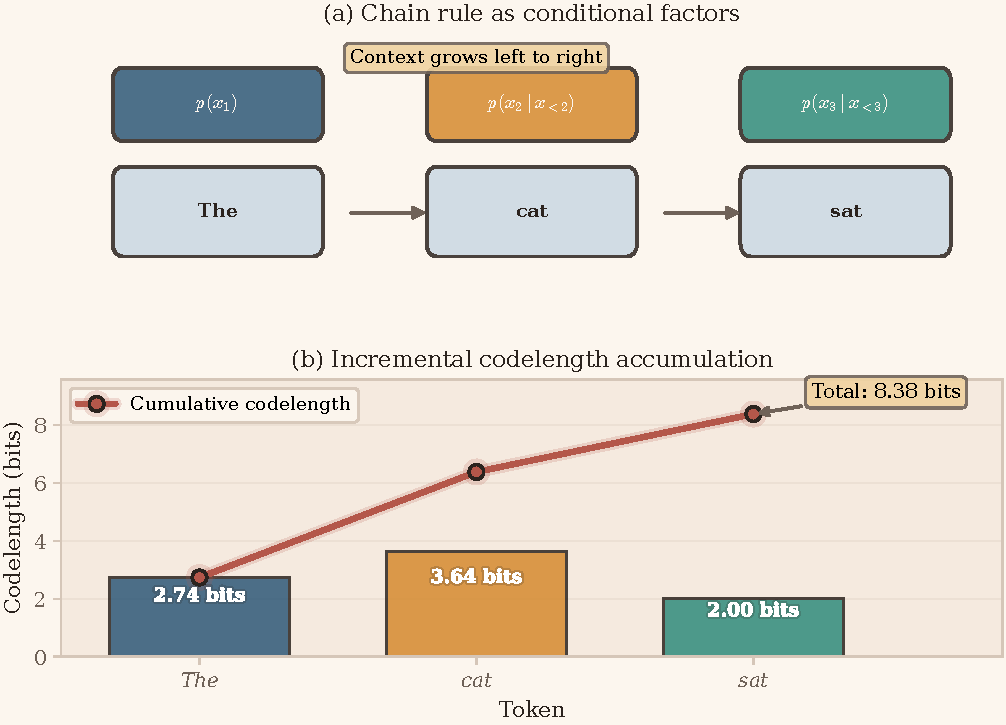
\includegraphics[width=0.95\textwidth]{code/figures/ch05_transformers_compressors/fig_5_1_autoregressive_factorization.pdf}
\caption{\textbf{Autoregressive factorization and incremental codelength.} Each next-token probability contributes additive bits to the total code.}
\label{fig:autoregressive_factorization}
\end{figure}
